\documentclass{article}
\usepackage[utf8]{inputenc}
\usepackage[a4paper, total={6in, 8in}]{geometry}
\usepackage{hyperref}
\usepackage{graphicx}
\hypersetup{
    colorlinks=true,
    linkcolor=blue,
    filecolor=magenta,      
    urlcolor=blue,
}

\title{Project Plan}
\author{Group 18}
\date{January 2021}

\begin{document}
\maketitle

\tableofcontents

\clearpage

\Large{\textbf{Abstract}}
\normalsize
\newline
Our product is a device that helps visually impaired users navigate their surroundings by using lidar technology to detect nearby objects and providing haptic feedback. 3 key milestones have been set up to monitor the progress in the vital functionality of the system. Firstly, by demo 1, having a reasonable lidar model and interpreting the lidar-obtained data in simulation. Secondly, by demo 2, having created a simple proof of concept tactile feedback device demonstrating its hardware feasibility. And lastly, by demo 3, having a functional prototype where the tactile feedback platform acts based on the lidar-obtained data. Each of these milestones is decomposed into a number of smaller subtasks, further divided into hardware and software components, and assigned to specific team members.
\section{Goal description}
Many people around the world suffer from visual impairment, which makes navigating the surrounding environment significantly challenging. To address this particular issue, we propose a device that uses a lidar to measure distances from nearby objects and provides haptic feedback to the user.

\subsection{Relevance of the system}
According to the World Health Organization (\href{https://www.who.int/blindness/publications/globaldata/en/#:~:text=Globally\%20the\%20number\%20of\%20people,blindness\%20is\%20cataract\%20(51\%25).}{WHO, 2010}), the number of people of all ages visually impaired is estimated to be 285 million, of whom 39 million are blind. As a result, different companies make several devices other than canes to help the visually impaired walk independently. However, these devices are either too expensive or are missing functionalities that would create a better user experience. Below, we have mentioned a couple that is a bit similar to our product.
\begin{itemize}
\item \href{https://wewalk.io/en/}{WeWalk} made a smart cane with an electronic handle and uses an ultrasonic sensor to detect any obstacles and warns the user via a vibrating handle. However, it only detects obstacles above the chest level and costs 500.


\item \href{https://italianinnovationday.weebly.com/horus-technology.html}{Horus Technology} made an ear-mounted device that observes and describes the environment to the person using it. However, this is very distracting to the user as it makes a continuous sound around obstacles and costs around 2000.
\end{itemize}
As so many technologies are coming out to the market tackling this vision problem, we believe that our product is marketable due to the affordability and various functionalities.
\newline
Our system tries to copy bats since they don’t have proper vision. We didn't’t use sound because there is too much sound pollution these days. We got the inspiration from (\href{https://www.youtube.com/watch?app=desktop&v=8Au47gnXs0w}{Stuff Made Here, 2020}) to use LIDAR to detect obstacles at a different distance from the user and translate that to haptic feedback to let the user beware of oncoming obstacles.


\subsection{High-level description}
We tried to find user stories by looking at relevant reports and interviews of visually impaired people, and formulated them into the followings:
\begin{itemize}
\item As a cane user, I want to get help with objects at body and head level as well so that I won't bump into a pole (\href{https://www.smithsonianmag.com/innovation/smart-cane-helps-blind-people-navigate-180973279/}{Smithsonian, 2019})
\item As a cane user, I want its symbolic function so people in busy environments such as airports will be more careful.(\href{https://link.springer.com/article/10.1007/s10209-020-00712-z}{SpringLink, 2020})
\item As a cane user, I want to detect objects far away so I wouldn’t be vulnerable to overhangs, such as tree branches.
\item I also want to detect objects under feet to help with drop-offs, like curbs and steps
\item As a cane user, I want object recognition so I can get around certain people, or find certain objects.
\item I want the cane to be lighter and more delicate so I can receive more information. (\href{https://whyy.org/segments/why-is-creating-electronic-canes-for-the-blind-so-hard/}{WHYY, 2019})
\item I want it to be simple to maintain so I don’t have to charge it or be worried that it would malfunction
\end{itemize} 
According to these, the major advantage of a smart device over the traditional cane is the ability to detect overhead objects, drop-offs, and far away objects. It should also be easy to use, simple to maintain, lightweight and responsive. The haptic feedback should be simple and it should not interfere with the normal cane usage. We aim to achieve as many of those in our product and would investigate further into the user experience.
\section{Task planning}

\subsection{Milestones}

The main subgoals that we are aiming for are successfully interpreting lidar data, creating a proof of concept tactile feedback device, and successfully translating lidar data to hardware. For the interpretation of lidar data, we would like to have that completed by the first demo, demonstrating that we have established our software foundation to build upon. We would like to have created a simple proof of concept tactile feedback device by the second demo to show that our hardware aspect is feasible. This would also include a simple demonstration of the lidar data being translated to an LED array to show that the software and hardware are communicating properly. Finally, we would like to fully translate our lidar data to the tactile feedback platform by the third demo to show that we have at least a simplified functional prototype. If possible we would also like to have a more complex tactile feedback device by then.

\subsection{Task Decomposition (Gantt)}
\begin{center}
    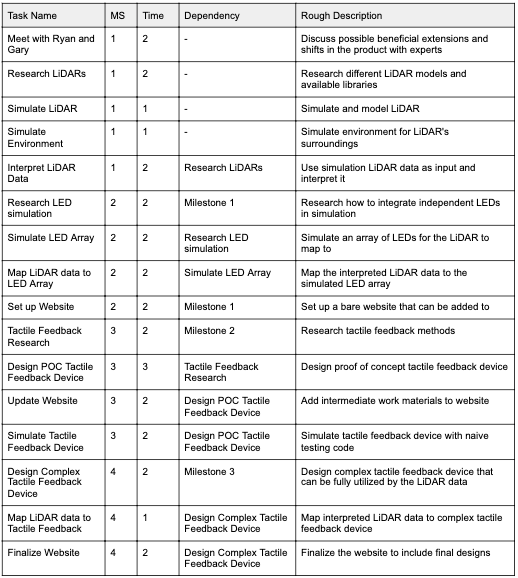
\includegraphics [width=0.7\textwidth]{Gantt.png}
\end{center}
\begin{center}
    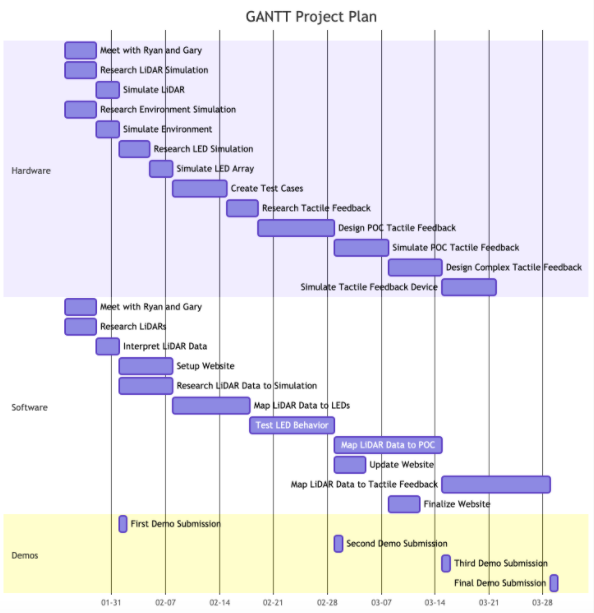
\includegraphics [width=0.7\textwidth]{Gantt PP.png}
\end{center}
\subsection{Resource distribution}
\subsubsection{Allocating Team Members Tasks}
On a high level description tasks in the Gantt chart were assigned to either the software team or the hardware team. From this we specify what task each member of the team is working on.
\begin{center}
    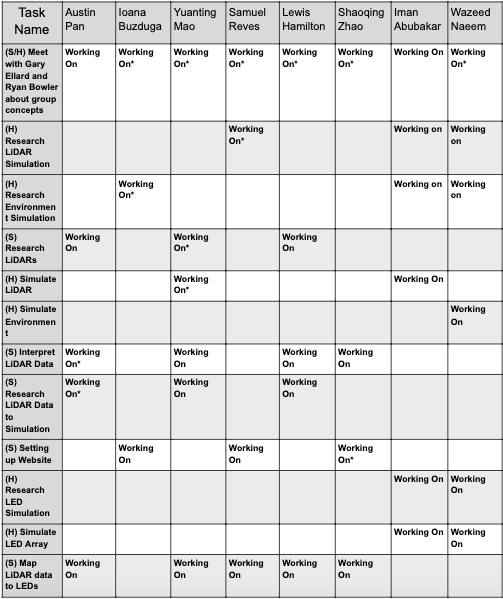
\includegraphics [width=0.68\textwidth]{Team Member Tasks 1.png}
    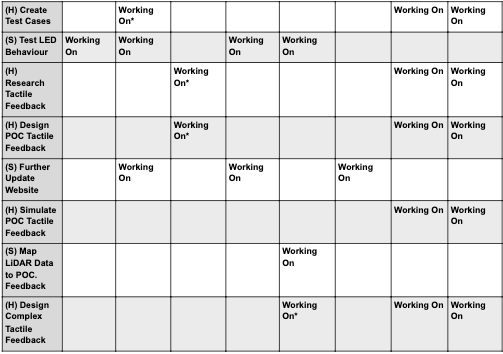
\includegraphics [width=0.68\textwidth]{Team Member Tasks2.png}
 \end{center}
H- Hardware task,
S- Software task 
\newline
The general idea of this table was to allocate a definite one or two people to each task in the Gantt chart. So for each week the team can look at the chart to see all the in progress tasks then consult this table to see which definite task they will be doing. 
\newline
Due to the imbalance in the group of people doing hardware/software as well as trying to adopt certain agile strategies, an asterisk (*) beside Working On for a task that they could also work on along with their definite task- an optional task. This allows for a more flexible use of resources if one task needs more people/work time on it than others as well as allowing certain software team members, who have hardware experience, to be involved in hardware if need be. For example if say Iman and Wazeed needed more time on the Create Test Cases task they could put up a ticket on Trello (discussed later in the report) which Ioana, whose optional task it is, could respond and help them with that task.  
\newline
It should be noted, while this section seems quite granular in its detail of who's doing what tasks, like many aspects of the project, this will be subject to change and more people may be given more optional tasks. This will both be updated in the table and using tickets on Trello. 
\subsubsection{Team Resources}
When allocating the tasks above, we took care to keep our teams resources in mind- particularly individual skills and strengths of each person. Listing our resources in terms of team members is reflective of the agile principle of ‘building the project around motivated individuals’ (\href{http://agilemanifesto.org/principles.html}{Agile Manifesto}) This is shown for example in Iman and Wazeed’s previous Hardware experience making them suitable for the Hardware Team and Austin’s previous start-up experience giving him the agile skills needed to head the Software Team. 
\begin{center}
    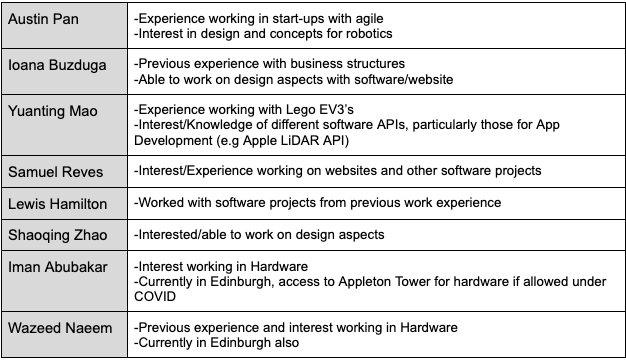
\includegraphics [width=0.7\textwidth]{Team Resources.png}
\end{center}
\subsection{Risk assessment}
\begin{center}
    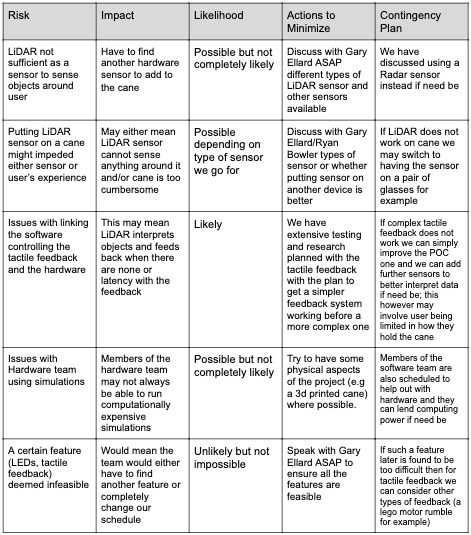
\includegraphics [width=0.7\textwidth]{Risk Assessment.png}
\end{center}
\section{Group organisation}
\subsection{Team Structure}
\begin{center}
    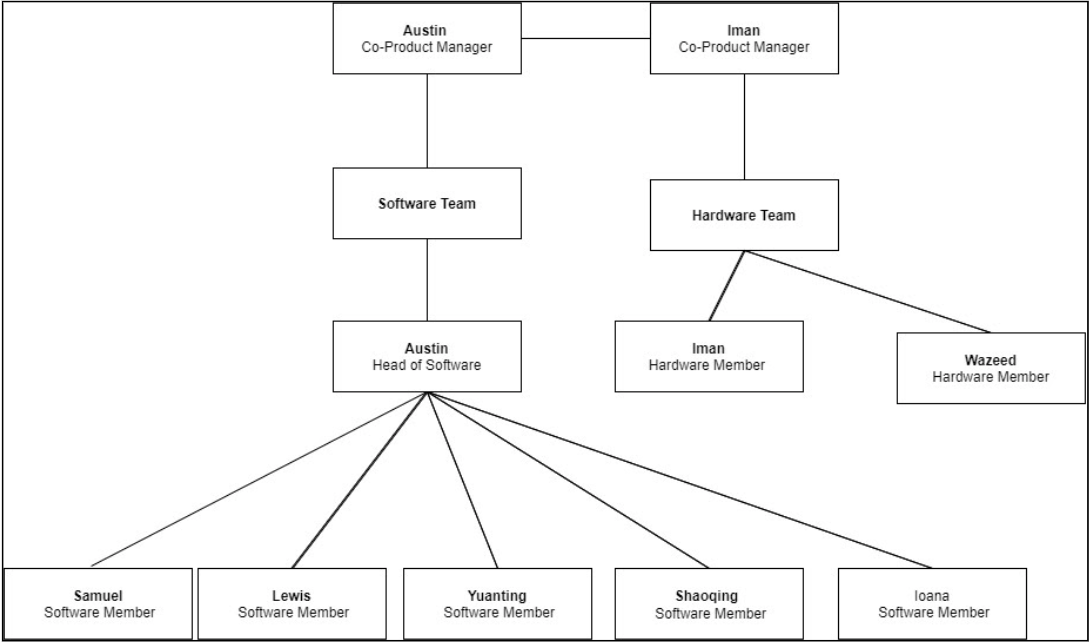
\includegraphics [width=0.7\textwidth]{Team Structure.png}
\end{center}
The above diagram explains the team structure. 
\newline
\textbf{Product Manager Responsibilities: }
\begin{enumerate} 
    \item Be the main point of contact between the team  and SDP teaching staff. 
    \item Keep track of the team's progress.
    \item Allocate tasks to the team. 
    \item Make sure the deadlines are met. 
    \item Make sure the team is keeping a good work ethic. 
    \item Conflict mediation, in case it appears. 
\end{enumerate}
\textbf{Head of Software Responsibilities: }
\begin{enumerate} 
    \item Allocate tasks within the Software team.
    \item Make sure the deadlines are met. 
    \item Keep track of progress.
    \item Conflict mediation, in case it appears in the Software team. 
\end{enumerate}
During next week, both the Software and Hardware team will choose roles and responsibilities within the team.

\subsection{Meetings}
The team decided to have a weekly meeting on Wednesdays at 2pm UK time as it is the most convenient time for everyone's respective time zone.The mentor will join the meeting. The time of the general meeting will be added as a calendar invite to the Outlook calendar of everyone. Ioana will do that.  At the general team meeting, everyone from the software and hardware team will share updates about their work progress and raise any concerns or suggestions. The hardware and software teams are welcomed to arrange meetings during that week to discuss the tasks related to their sector. At the general team meetings, Ioana will be in charge of taking the minutes and uploading them on the shared drive. 

\subsection{Official Communication with the Team}
The general communication with the entire members of the team will be on a Teams group chat. 
\newline
\textbf{The reasons for opting for a Teams group chat are: }
\begin{itemize}
\item It is on the same platform as the one used for the course. 
\item The chat allows the function to share files, call both with or without video, and share screen. 
\item The chat allows the option to organise polls. 
\item Different applications can be embedded in the chat. For example, a Trello extension has been added to the chat. This will help with task allocation and tracking. 
\end{itemize}
The Software team decided to create a separate chat for communicating software-related tasks as the Software team is formed of 6 people and the hardware team of 2. Everyone will join that chat. 

\subsection{Code Sharing}
The code will be shared by using a Github repository. The decision was taken, because everyone from the team is familiar with using Github The repository will be made private and Austin has already created and shared it with the entire team.  
\newline
\textbf{Benefits of using Github: }
\begin{itemize}
\item Easy to track changes. 
\item Github can integrate platforms such as Amazon and Google Clouds. 
\item The code is safely stored in case of computer damage. 
\end{itemize}
\subsection{Task Allocation and Progress Tracking}
The team decided to use Trello for both task allocation and tracking. 
\newline 
\textbf{Reasons for using Trello:}
\begin{itemize}
\item Creating multiple boards,unique to each subteam.
\item Adding due dates for each task
\item Assigning team members to each task
\item Splitting the tasks into low, high priority or urgent tasks.
\item Incorporating to the Teams group chat. 
\item Splitting the tasks into different subcategories: To Do, In Progress, Struggling and Done. 
\item Easing the process of tracking.
\item User-friendly. 
\end{itemize}
\textbf{Why is Trello useful for Agile Workflows? }
\newline
\newline
Agile development implies  that large projects are split into smaller chunks. The tasks are classified based on prioritization. The groups of tasks are executed in continuous iterations, which are coordinated across different sub-sectors or teams ( in our case, between Software and Hardware teams .Tasks can be easily re-prioritized and moved around as the need arises.(\href{https://blog.hubstaff.com/agile-trello/#:~:text=Because\%20it's\%20so\%20easy\%20to,stages\%2C\%20roles\%2C\%20and\%20deadlines.}{HubstaffBlog, 2019})
\newline
Trello enables the tasks to be re-prioritized, moved around different subcategories (e.g To Do, In Progress, Struggling and Done), add members of a different subteam to that task, create a color labelling system  and track time on tasks. 

\subsubsection{Task Allocation}

Austin will be in charge allocating the  tasks. The team decided to use Trello for task allocation. The Trello has already been created and the board with tasks was shared with everyone from the team. 

\subsubsection{Progress Tracking}

Trello will be used for progress tracking as well. Each task will have a due date and 1 to 2 team members assigned to it. The members have the responsibility to move the task one the categories: To Do, In Progress, Struggling,Done. During the team meetings, we will decide whether each ongoing task is high or low priority. At the end of each week,Ioana will archive all the tasks under the Done category.






\end{document}
